\documentclass[10pt, leqno]{amsart}

\usepackage{algorithm}
\usepackage[noend]{algpseudocode}
\usepackage{amsfonts}
\usepackage{amsmath}
\usepackage{amssymb}
\usepackage{amsthm}
\usepackage[backend=biber, citestyle=numeric-comp, bibstyle=ieee]{biblatex}
\usepackage{changepage}
\usepackage{enumitem}
\usepackage{fancyhdr}
\usepackage{fontspec}
\usepackage{fullpage}
\usepackage[hidelinks]{hyperref}
\usepackage{marvosym}
\usepackage{mathtools}
\usepackage[]{mdframed}
\usepackage{physics}
\usepackage[skins]{tcolorbox}
\usepackage{thmtools}

\usepackage{tikz-3dplot}
\usetikzlibrary{angles, calc, cd, quantikz, quotes, patterns}
\usepackage{titlesec}
\usepackage{wasysym}

\usepackage{tikz-cd}

\usepackage{bookmark}
\usepackage[nameinlink]{cleveref}

\titleformat{\section}[runin]{\normalsize\bfseries}{\thesection}{1em}{}[]
\titleformat{\subsection}[runin]{\normalsize\bfseries}{\thesubsection}{1em}{}[]
\titleformat{\subsubsection}[runin]{\normalsize\bfseries}{\thesubsubsection}{1em}{}[]

\addbibresource{convex_analysis_subdifferentials_and_the_finite_dimensional_real_situation_handout.bib}

\theoremstyle{definition}
\newtheorem{theorem}{Theorem}[section]
\newtheorem{conjecture}{Conjecture}[section]
\newtheorem{definition}{Definition}[section]
\theoremstyle{remark}
\newtheorem{problem}[theorem]{Problem}
\newtheorem{lemma}[theorem]{Lemma}
\newtheorem{remark}[theorem]{Remark}
\newtheorem{observation}[theorem]{Observation}
\newtheorem{example}[theorem]{Example}
\newtheorem{corollary}[theorem]{Corollary}

\renewcommand{\qedsymbol}{\(\blacksquare\)}

\setlength{\parindent}{0pt}

\renewcommand{\theequation}{\arabic{equation}}
\renewcommand{\thetheorem}{\arabic{theorem}}

\DeclareMathOperator{\controrot}{CR}
\DeclareMathOperator{\expectation}{E}
\DeclareMathOperator{\gf}{GF}
\DeclareMathOperator{\qft}{QFT}
\DeclareMathOperator{\rk}{rk}
\DeclareMathOperator{\defect}{def}
\DeclareMathOperator{\swapgate}{SWAP}
\DeclareMathOperator{\che}{CHE}
\DeclareMathOperator{\poly}{poly}
\DeclareMathOperator{\Span}{Span}
\DeclareMathOperator{\diag}{diag}

\newcommand{\djk}{\delta_{j, k}}
\newcommand{\tlk}{\tilde{\lambda_k}}

\newcommand{\evalat}[2]{\left.{#1}\middle|\right._{#2}}

% SOURCE: https://tex.stackexchange.com/questions/296151/double-head-and-hook-arrow
\newcommand{\hookdoubleheadrightarrow}{%
  \hookrightarrow\mathrel{\mspace{-15mu}}\rightarrow
}

\newtcolorbox{edgebox}{enhanced, colback=white, frame code={%
\draw[very thin] (frame.north west) -- ($(frame.north west) + ( 0.5, 0)$);
\draw[very thin] (frame.north west) -- ($(frame.north west) + (0, -0.5)$);
\draw[very thin] (frame.south east) -- ($(frame.south east) + (-0.5, 0)$);
\draw[very thin] (frame.south east) -- ($(frame.south east) + (0,  0.5)$);
}}

\AtEveryBibitem{%
  \clearfield{journaltitle}%
  \clearfield{date}%
  \clearfield{volume}%
  \clearfield{pages}%
  \clearfield{publisher}%
  \clearfield{number}%
  \clearfield{journaltitle}%
}

\newcommand{\commentcmd}[1]{}

\newcommand{\draftcommenttodo}{\textcolor{red}{ TODO }}
\newcommand{\draftcommentdone}{\textcolor{green}{ DONE }}

\begin{document}
    \pagenumbering{gobble}

    \begin{mdframed}
        \textsc{Seminar on Convex Analysis} \hfill valentinpi\\
        Freie Universität Berlin \hfill July 25, 2023\\
        Summer Term 2023
    \end{mdframed}

    \section*{Presentation Handout on: Further Properties of Subdifferentials and The Situation in \(\mathbb{R}^n\)}

    \phantom{}

    \begin{theorem}[{\textbf{A Chain Rule} \cite[p. 201]{IoffeTihomirov}}]
        Let \(\Lambda \in L(X, Y)\) and \(f\colon Y \to \overline{\mathbb{R}}\) be a function.
        \begin{enumerate}[label=(\roman*), wide]
            \item \label{compat_with_operator_theorem_1} For any \(x \in X\), we have
            \begin{align}
                \partial (f\Lambda)(x) \supseteq \Lambda^*\partial f(\Lambda x)
            \end{align}
            \item \label{compat_with_operator_theorem_2} If \(f\) is convex and proper on \(X\), as well as continuous at a point in \(\text{Im}(\Lambda)\), then for any \(x \in X\)
            \begin{align}
                \partial (f\Lambda)(x) = \Lambda^*\partial f(\Lambda x) \label{compat_with_operator_theorem_eq_2}
            \end{align}
        \end{enumerate}
    \end{theorem}

    \begin{figure}[!hbtp]
        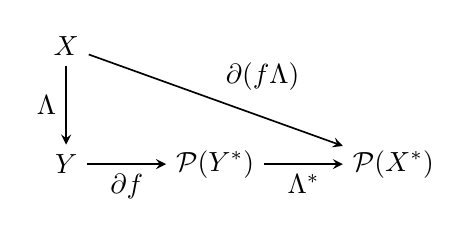
\begin{tikzpicture}[>=stealth, semithick]
            \node (0) at (0, 0) {\(X\)};
            \node[below=1cm of 0] (1) {\(Y\)};
            \node[right=1cm of 1] (2) {\(\mathcal{P}(Y^*)\)};
            \node[right=1cm of 2] (3) {\(\mathcal{P}(X^*)\)};
            \draw[->] (0) -- (1) node[left, pos=0.5] {\(\Lambda\)};
            \draw[->] (1) -- (2) node[below, pos=0.5] {\(\partial f\)};
            \draw[->] (2) -- (3) node[below, pos=0.5] {\(\Lambda^*\)};
            \draw[->] (0) -- (3) node[above right, pos=0.5] {\(\partial (f\Lambda)\)};
        \end{tikzpicture}
    \end{figure}

    \begin{theorem}[{\textbf{Supremum Functions} \cite[pp. 201-204]{IoffeTihomirov}}] \label{supremum_theorem}
        Let \(S\) be a compact topological space and \(f\colon S \times X \to \overline{\mathbb{R}}\), s.t. for any \((s, x) \in S \times X\), \(f|_{\{s\} \times X}\) is convex and proper, and that \(f|_{S \times \{x\}}\) is upper semicontinuous, where we each omit the respective fixed argument. Let \(f_s \coloneqq f|_{\{s\} \times X}\) and set
        \begin{align}
            \hat{f}\colon X \to \overline{\mathbb{R}}, x \mapsto \sup_{s \in S} f_s(x) \text{ and } S_0\colon X \to \mathcal{P}(S), x \mapsto \{s \in S \mid f_s(x) = \hat{f}(x)\}.
        \end{align}
        In both of the following statements, the closures are taken wrt. the weak\({}^*\)-topology of \(X^*\).
        \begin{enumerate}[label=(\roman*), wide]
            \item \label{supremum_theorem_1} For any \(x \in X\)
            \begin{align}
                \overline{\text{conv}}\left(\bigcup_{s \in S_0(x)} \partial f_s(x)\right) \subseteq \partial \hat{f}(x)
            \end{align}
            \item \label{supremum_theorem_2} If for all \(s \in S\), \(f_s\) is continuous at a point \(x_0 \in X\), then
            \begin{align}
                \overline{\text{conv}}\left(\bigcup_{s \in S_0(x_0)} \partial f_s(x_0)\right) = \partial \hat{f}(x_0)
            \end{align}
        \end{enumerate}
    \end{theorem}

    Let \(n \in \mathbb{N}_{\geq 1}\).

    \begin{theorem}[{\cite[p. 204]{IoffeTihomirov}}]
        Let \(f\colon \mathbb{R}^n \to \overline{\mathbb{R}}\) be proper and convex. Then \(f\) is subdifferentiable in \(\text{ri}(\text{dom}(f))\).
    \end{theorem}

    \begin{theorem}[{\cite[pp. 204-205]{IoffeTihomirov}}] \label{finite_dim_representation_theorem}
        Let \(X, S, f, f_s, \hat{f}, S_0, x_0\) for \(X = \mathbb{R}^n\) and any \(s \in S\) be defined as in the setting of \Cref{supremum_theorem} \ref{supremum_theorem_2}. Then every \(y \in \partial \hat{f}(x_0)\) can be represented as a convex combination of form
        \begin{align}
            y = \sum_{i=1}^r \alpha_i y_i
        \end{align}
        with \(r \in \mathbb{N}\), \(1 \leq r \leq n+1\), \(\sum_{i=1}^r \alpha_i = 1\) and \(s_i \in S_0(x_0)\), \((\alpha_i, y_i) \in \mathbb{R}_{>0} \times \partial f_{s_i}(x_0)\) for any \(i \in \mathbb{N}\), \(1 \leq i \leq r\).
    \end{theorem}

    \printbibliography{}
\end{document}
